\documentclass[aspectratio=43,10pt]{beamer}

%% ─── Theme ────────────────────────────────────────────────────────
\usetheme[iut, sans, progressbar=segmented, nosub]{Shibui}

%% ─── Packages ────────────────────────────────────────────────────
\usepackage[utf8]{inputenc}
\usepackage[T1]{fontenc}
\usepackage[french]{babel}
\usepackage{listings}
\usepackage{translator}
\uselanguage{French}
\languagepath{French}
\usepackage{graphicx}
\usepackage{tikz}
\usepackage{pgfplots}
\pgfplotsset{compat=1.18}
\usetikzlibrary{arrows.meta,positioning,calc}
\usepgfplotslibrary{fillbetween,groupplots}

\graphicspath{{../../../common/figures/ch1/}}
\usepackage{amsmath,amsfonts,bm}

%% ─── Operators ───────────────────────────────────────────────────
\DeclareMathOperator*{\argmax}{arg\,max}
\DeclareMathOperator*{\argmin}{arg\,min}
\DeclareMathOperator{\MSE}{MSE}
\DeclareMathOperator{\sign}{sign}
\DeclareMathOperator{\sinc}{sinc}
\DeclareMathOperator{\tr}{tr}

%% ─── Number sets ─────────────────────────────────────────────────
\def\R{{\mathbb{R}}}
\def\C{{\mathbb{C}}}
\def\N{{\mathbb{N}}}
\def\Z{{\mathbb{Z}}}

%% ─── Infinitesimal and units ────────────────────────────────────
\def\d{{\rm d}}
\def\Hz{{\mbox{Hz}}}
\def\m{{\mbox{m}}}

%% ─── Complex / signal ───────────────────────────────────────────
\DeclareMathOperator{\complexj}{\mathsf{j}}   % imaginary unit

%% ─── Probability ─────────────────────────────────────────────────
\newcommand{\Esp}[2]{\mathbb{E}_{#1}\!\left[#2\right]}
\renewcommand{\Pr}{\mathbb{P}}

%% ─── Linear algebra ──────────────────────────────────────────────
\newcommand{\abs}[1]{\left|{#1}\right|}
\newcommand{\norm}[1]{\left\|#1\right\|}
\newcommand{\inner}[2]{\left\langle#1,\,#2\right\rangle}

%% ─── Logic ───────────────────────────────────────────────────────
\newcommand{\then}{\Rightarrow}
\newcommand{\iif}{\Leftrightarrow}

%% ─── Draft annotation ────────────────────────────────────────────
\newcommand{\red}[1]{{\color{red}#1}}

%% ─── Shared figure color (used by common/figures/*/*.tex bodies) ──
\definecolor{niceblue}{RGB}{0,128,172}

%% ─── Rappel header (styled subtitle for reference-card asides) ───
%% Requires \definecolor{niceblue}{...} to be defined by the including document.
\newcommand{\rappelhead}[1]{%
    \bigskip
    {\color{niceblue}\bfseries #1}\\[-0.4em]
    {\color{niceblue!35}\rule{\linewidth}{0.6pt}}
    \smallskip

}


%% ─── Metadata ─────────────────────────────────────────────────────
\title{Outils Mathématiques et Logiciel --- OML3}
\subtitle{Chapitre 1 --- Série de Fourier}
\author{\textbf{BUT2} -- Génie Électrique et Informatique Industrielle}
\date{2025-2026}

%% ─── Theorem environments ─────────────────────────────────────────
%% `definition` and `theorem` are already provided (and auto-localized
%% via babel) by the beamer class itself -- only declare the extra ones.
\newtheorem{proposition}{Propriété}
\newtheorem{remark}{Remarque}

%% ─── Text helper (mirrors poly/main.tex) ───────────────────────────
\newcommand{\highlight}[1]{{\color{niceblue}\emph{#1}}}

%% ─── Figure helper : fit any \input'd figure to a target width ────
\newcommand{\slidefig}[2]{%
\begin{center}
\resizebox{#1}{!}{\input{../../../common/figures/ch1/#2}}
\end{center}
}

%% ─────────────────────────────────────────────────────────────────
\begin{document}
\shorthandoff{:;!?}

\maketitle

%% ═══════════════════════════════════════════════════════════════════
%% SÉANCE 1 (CM1) : sections "Rappels", "Fonctions périodiques",
%%                   "Série de Fourier" (forme trigonométrique)
%% SÉANCE 2 (CM2) : section "Forme complexe"
%% Mirrors poly/main.tex — same running example (signal créneau).
%% ═══════════════════════════════════════════════════════════════════

%% ─── SECTION : Rappels ──────────────────────────────────────────
\section{Rappels}

\begin{frame}{Notations}
    \begin{center}
    \renewcommand{\arraystretch}{1.3}
    \begin{tabular}{cl}
        $\R$ & ensemble des nombres réels \\
        $\C$ & ensemble des nombres complexes \\
        $\N$ & ensemble des entiers naturels \\
        $\Z$ & ensemble des nombres entiers relatifs \\
        $\forall x\in\R$ & « pour tout $x$ réel » \\
        $\exists T\in\N$ & « il existe $T$ entier » \\
        $E^*$ & $E\setminus\{0\}$
    \end{tabular}
    \end{center}
\end{frame}

\begin{frame}{Sommes et suites}
    \begin{definition}[Somme]
        Pour une suite $(u_k)$ et deux entiers $m\leq n$,
        \[
            \sum_{k=m}^{n} u_k = u_m + u_{m+1} + \cdots + u_n.
        \]
    \end{definition}
    \[
        \sum_{k=1}^{N} k = 1+2+\cdots+N = \frac{N(N+1)}{2}
    \]
    \[
        \sum_{k=1}^{N} 3^k = 3+3^2+\cdots+3^N = \frac{3\left(3^N-1\right)}{2}
    \]
\end{frame}

\begin{frame}{Séries}
    % \begin{definition}[Série]
         La série de somme partielle $S_N$ \highlight{converge} si $$S_N=\sum_{n=0}^{N}u_n \underset{N\to +\infty}{\longrightarrow} S$$
          Sinon elle \highlight{diverge}.
    % \end{definition}
    \slidefig{\textwidth}{series-convergence.tex}
    \begin{center}
        \small
        $\displaystyle\sum \frac1k$ diverge, mais
        $\displaystyle\sum \frac1{k^2}=\frac{\pi^2}{6}$ converge.
    \end{center}
\end{frame}

\begin{frame}{Rappels sur l'intégrale}
    \[
        \int_a^b f(t)\,\d t = F(b)-F(a), \qquad F^\prime=f
    \]

    
    \only{\slidefig{.5\textwidth}{integral-area.tex}
        \begin{center}
        \small Pour $f(x)=\alpha x$ :
        $\displaystyle\int_a^b \alpha x\,\d x = \frac{\alpha}{2}\left(b^2-a^2\right)$
        \end{center}
        }<1>


        \only{
        \begin{center}
        \textbf{Chasles}\\[0.5em]
        $\displaystyle\int_a^c f = \int_a^{\red{b}} f + \int_{\red{b}}^c f$
    \end{center}
        }<2>

        \only{
        \begin{center}
        \textbf{Linéarité}\\[0.5em]
        $\displaystyle\int_a^b(\red{f}+{\color{niceblue}g}) = \int_a^b \red{f} + \int_a^b {\color{niceblue}g}$\\[0.4em]
        $\displaystyle\int_a^b \red{\lambda} f = \red{\lambda}\int_a^b f$
        \end{center}
        }<3>

        \only{
        \begin{center}
        \textbf{Parité}\\[0.5em]
        $f$ paire $\Rightarrow \displaystyle\int_{-a}^a f = 2\int_0^a f$ \qquad
        $f$ impaire $\Rightarrow \displaystyle\int_{-a}^a f = 0$
        \end{center}
        \slidefig{0.7\textwidth}{integral-parity.tex}
        }<4>
\end{frame}

%% ─── SECTION : Fonctions périodiques ────────────────────────────
\section{Fonctions périodiques}

\begin{frame}{Fonction périodique}
    \begin{definition}[Fonction périodique]
        $f$ est $T$-périodique si $$\forall x\in\R, \exists T > 0, \quad f(x+T)=f(x).$$
        Fréquence $f_0=1/T$, pulsation $\omega_0=2\pi f_0$.
    \end{definition}
    \slidefig{\textwidth}{periodic-examples.tex}
\end{frame}

\begin{frame}{Propriétés des fonctions périodiques}
    \begin{proposition}[Somme de fonctions périodiques]
        Si $f$ est $T$-périodique et $g$ est $T^\prime$-périodique, avec
        $p,q\in\N^*$ tels que $pT=qT^\prime$, alors $f+g$ est
        périodique, de période le ppcm de $T$ et $T^\prime$.
    \end{proposition}
        \small
        \begin{exampleblock}{Exemple}
        $\sin(2\pi t \times \frac{1}{2})$ est $2$-périodique, $\sin(2\pi t \times \frac{1}{3})$
        est $3$-périodique. Leur somme est $6$-périodique (ppcm de $2$
        et $3$).
        \end{exampleblock}
        % \begin{alertblock}{Remarque}
        % Si $T/T^\prime$ est irrationnel, la somme n'est en général pas
        % périodique.
        % \end{alertblock}
        \slidefig{\textwidth}{periodic-sum-example.tex}
\end{frame}

\begin{frame}{Cosinus et sinus}
    \begin{columns}
        \column{0.62\textwidth}
        \slidefig{\textwidth}{trig-cos-sin.tex}
        \column{0.34\textwidth}
        \slidefig{\textwidth}{unit-circle.tex}
    \end{columns}
    \begin{columns}
        \column{0.5\textwidth}
        \[
            \sin(t) = \cos\!\left(t-\frac{\pi}{2}\right)
        \]
        \column{0.5\textwidth}
        \[
            \cos^2(t)+\sin^2(t)=1
        \]
    \end{columns}
\end{frame}

\begin{frame}{Formules à connaître}
    \begin{proposition}[Addition]
        \[
            \cos(a+b)=\cos a\cos b - \sin a\sin b, \qquad
            \sin(a+b)=\sin a\cos b + \cos a\sin b
        \]
    \end{proposition}
    \begin{proposition}[Somme-produit]
        \[
            \cos p+\cos q = 2\cos\!\Big(\tfrac{p+q}{2}\Big)\cos\!\Big(\tfrac{p-q}{2}\Big),
            \qquad
            \sin p+\sin q = 2\sin\!\Big(\tfrac{p+q}{2}\Big)\cos\!\Big(\tfrac{p-q}{2}\Big)
        \]
    \end{proposition}
\end{frame}

\begin{frame}{Application : quelle est la période ?}
    \[
        f(t) = \cos(2\pi \times 440 \times t)
    \]
    \begin{center}\small Quelle est la période de $f$ ?\end{center}
    \vspace{1.5em}
    \[
        g(t) = \cos(2\pi f_1 t)\,\cos(2\pi f_2 t)
    \]
    \begin{center}
        \small Quelle est la période de $g$ ?
    \end{center}
\end{frame}

\begin{frame}{Signaux périodiques usuels}
    \begin{overprint}
    \onslide<1>
    $$
        f_{\rm carr\acute{e}}(t) = \begin{cases} 1 & \text{pour} \ t \in [kT,kT + \frac{T}{2}[, \ k\in\Z\\ -1 & \text{pour} \ t \in [kT + \frac{T}{2},kT[, \ k\in\Z \end{cases}
    $$
    \slidefig{0.6\textwidth}{signal-carre-slide.tex}
    \begin{center}\small Signal carré\end{center}
    \onslide<2>
    $$
    f_{\rm triangle}(t) = \begin{cases} t & \text{pour} \ t - kT \in [kT,kT + \frac{T}{2}], \ k\in\Z\\ (k+1)T - t & \text{pour} \ t \in [kT + \frac{T}{2},kT], \ k\in\Z \end{cases}
    $$
    \slidefig{0.6\textwidth}{signal-triangle-slide.tex}
    \begin{center}\small Signal triangle --- c'est l'intégrale du signal carré\end{center}
    \onslide<3>
    $$
    f_{\rm scie}(t) = t - kT ,\ k\in\Z
    $$
    \slidefig{0.6\textwidth}{signal-scie-slide.tex}
    \begin{center}\small Dents de scie\end{center}
    \end{overprint}
\end{frame}

\begin{frame}{Peut-on analyser systématiquement un signal périodique ?}
    \begin{columns}
        \column{0.5\textwidth}
        \begin{center}\small Somme de deux sinus\end{center}
        \slidefig{\textwidth}{signal-composite.tex}
        \column{0.5\textwidth}
        \begin{center}\small Signal périodique quelconque\end{center}
        \slidefig{\textwidth}{signal-chaotic.tex}
    \end{columns}
    \begin{alertblock}{Question}
        Existe-t-il une méthode systématique pour décrire n'importe
        quel signal périodique par une somme de fonctions périodiques ?
    \end{alertblock}
\end{frame}

%% ─── SECTION : Série de Fourier ─────────────────────────────────
\section{Série de Fourier}

\begin{frame}{Série trigonométrique}
    \begin{overprint}

    \begin{definition}[Série trigonométrique]
        \[
            \red{a_0} + \sum_{n=1}^{+\infty}\left(\red{a_n}\cos(n\omega_0 t)+\red{b_n}\sin(n\omega_0 t)\right)
        \]
    \end{definition}

    \begin{exampleblock}{Exemples}
        \small
        $\sin(t) \to \quad a_0=0,\ a_n=0\ \forall n,\ b_1=1,\ b_n=0\ (n>1)$
        \\[1em]
        $f(t)=4+\cos\!\left(2\pi f t+\dfrac{\pi}{2}\right) \to a_0=4,\ a_1=0,\ b_1=-1,\ a_n=b_n=0\ (n>1)$
    \end{exampleblock}
    \begin{alertblock}{Attention}
        Rien ne garantit a priori qu'une série trigonométrique converge.
    \end{alertblock}
    \end{overprint}
\end{frame}

\begin{frame}{Joseph Fourier (1807)}
    \begin{columns}
        \column{0.38\textwidth}
        \begin{center}
        \begin{figure}
            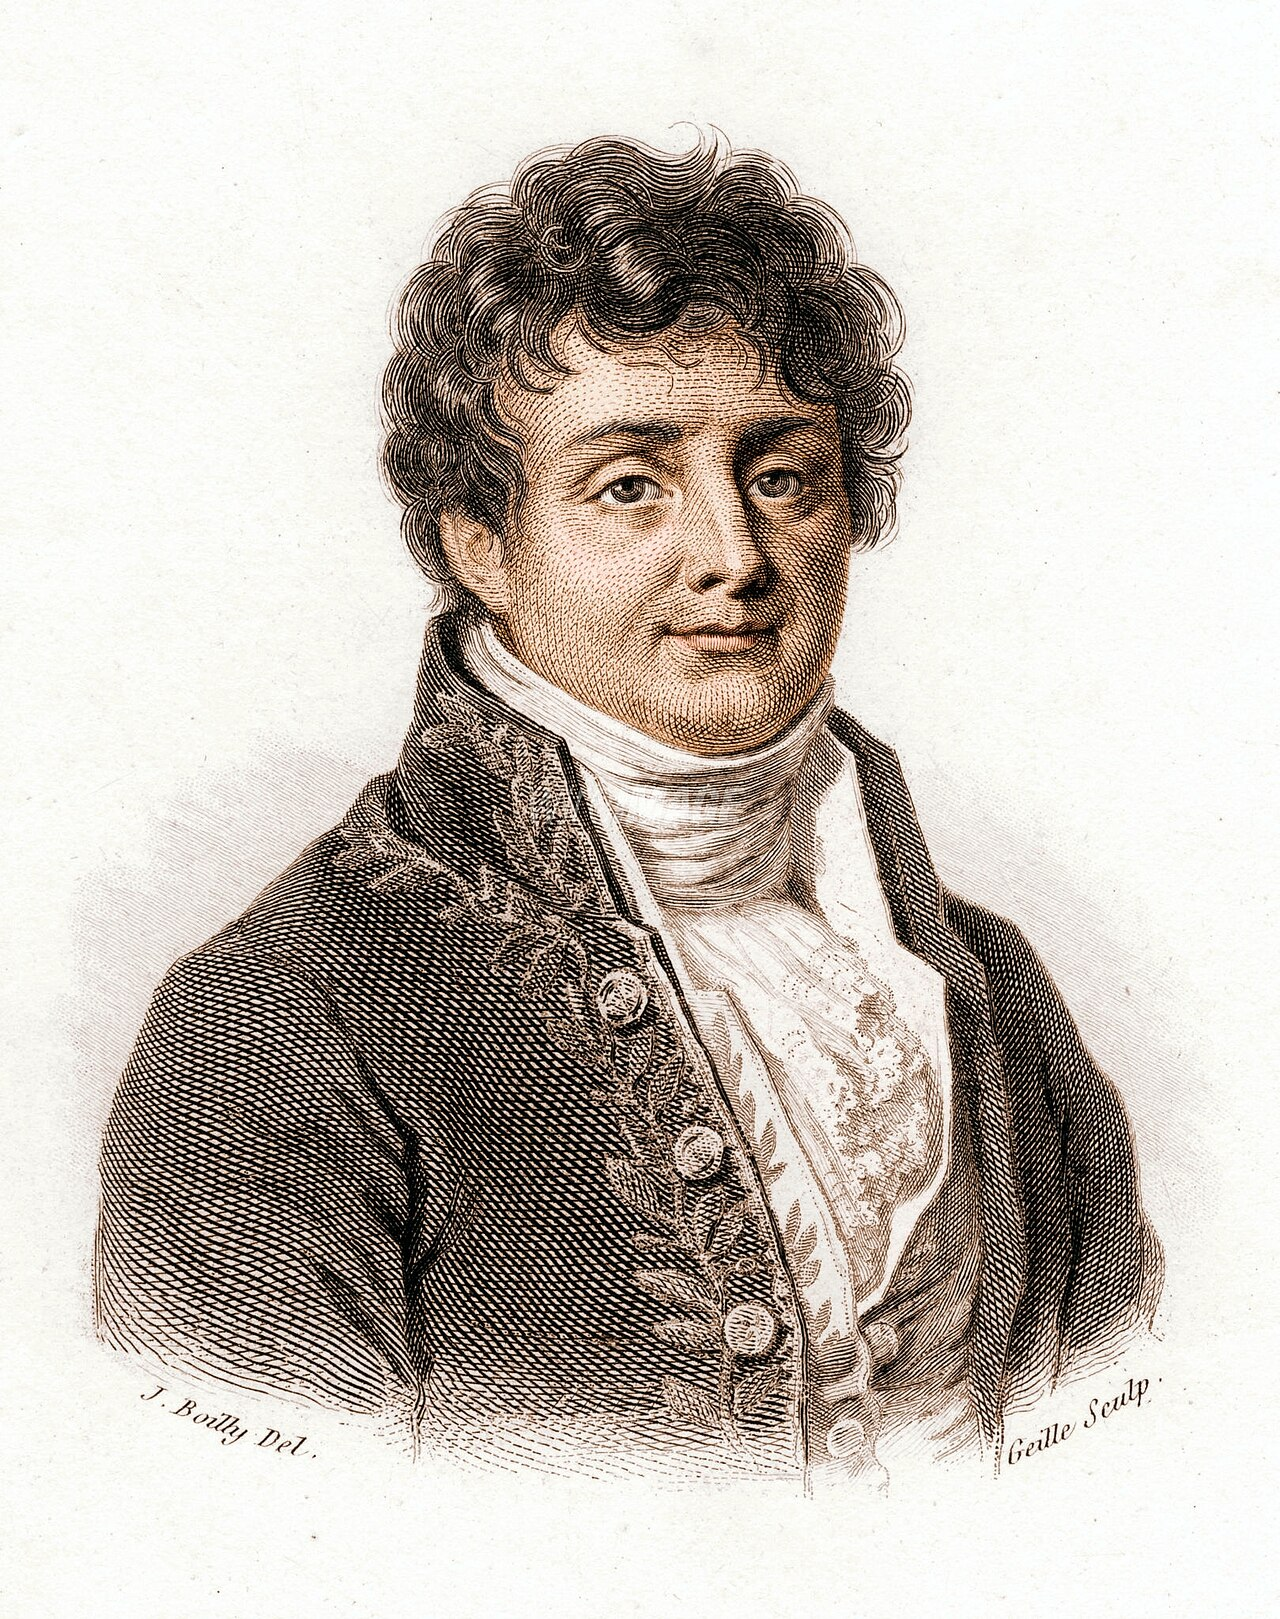
\includegraphics[width=0.8\textwidth]{fourier.jpg}
            \caption{Portait de Joseph Fourier}
        \end{figure}
        \end{center}
        \column{0.62\textwidth}
        % \slidefig{\textwidth}{fourier-heatbar.tex}
    \end{columns}
    \begin{center}
        \small Fourier étudie la diffusion de la chaleur dans une barre
        --- et montre qu'une fonction périodique se décompose en somme
        de sinusoïdes.
    \end{center}
\end{frame}

\begin{frame}{Théorème de Fourier}
    \begin{overprint}
    \onslide<1>
    \begin{theorem}[Développement en série de Fourier]
        Si $f$ est $T$-périodique et vérifie les conditions de
        Dirichlet,
        \[
            f(t) = a_0 + \sum_{n=1}^{+\infty}\left(a_n\cos(n\omega_0 t)+b_n\sin(n\omega_0 t)\right)
        \]
    \end{theorem}
    \[
        a_0 = \frac1T\int_0^T f(t)\,\d t
    \]
    \[
        a_n = \frac2T\int_0^T f(t)\cos(n\omega_0 t)\,\d t, \qquad
        b_n = \frac2T\int_0^T f(t)\sin(n\omega_0 t)\,\d t
    \]
    \onslide<3>
    \small
    \begin{definition}[Conditions de Dirichlet]
        Sur une période, $f$ vérifie :
        \begin{itemize}
            \item un nombre fini de discontinuités (sauts finis) ;
            \item un nombre fini d'extrema ;
            \item $f$ est bornée.
        \end{itemize}
    \end{definition}
    \slidefig{\textwidth}{dirichlet-example.tex}
    \onslide<2>
    \slidefig{\textwidth}{fourier-partial-sums.tex}
    \begin{center}
        \small Signal carré (noir) et son approximation par $N=1$, $5$, $9$
        harmoniques.
    \end{center}
    \end{overprint}
\end{frame}

\begin{frame}{$a_0$ : la composante continue}
    \[
        f(t) = a_0 + \sum_{n=1}^{+\infty}\left(a_n\cos(n\omega_0 t)+b_n\sin(n\omega_0 t)\right),
        \qquad
        a_0 = \frac1T\int_0^T f(t)\,\d t
    \]
    \slidefig{0.6\textwidth}{dc-mean.tex}
    \begin{center}
        \small $a_0$ est la valeur moyenne de $f$ sur une période ---
        ce que mesurerait un voltmètre en position DC.
    \end{center}
\end{frame}

\begin{frame}{Propriétés des coefficients --- linéarité}
    \begin{proposition}[Linéarité]
        Les coefficients de $\lambda f + \mu g$ sont
        $(\lambda a_n+\mu a_n^\prime,\ \lambda b_n+\mu b_n^\prime)$.
    \end{proposition}
    \begin{exampleblock}{Exemple}
        $f=\cos(\omega_0 t) \to a_1=1$ et
        $g=\sin(\omega_0 t) \to b_1=1$, alors 
        $$f+2g  \to a_1=1, b_1=2$$ 
    \end{exampleblock}
\end{frame}

\begin{frame}{Propriétés des coefficients --- parité}
        \begin{proposition}[Parité]
            $f$ paire $\Rightarrow \forall n \ b_n=0$  (série de cosinus).
            \\[1em]
            $f$ impaire $\Rightarrow  a_0=0,\ \forall n \ a_n=0\ $  (série de sinus).
        \end{proposition}
        \slidefig{\textwidth}{parity-illustration.tex}
\end{frame}

\begin{frame}{Spectre d'amplitude}
    \small
    \begin{definition}[Spectre d'amplitude]
        Pour $n\geq1$ on note la puissance associé au rang $n$, $$A_n=\sqrt{a_n^2+b_n^2}$$
    \end{definition}

    Exemple : spectre de $f(t)=2\cos(\omega_0 t)+\sin(2\omega_0 t)$
    \[
        a_1=2,\ b_1=0 \Rightarrow A_1=2 \qquad\qquad
        a_2=0,\ b_2=1 \Rightarrow A_2=1
    \]
    \slidefig{0.55\textwidth}{spectre-simple-example.tex}
\end{frame}

\begin{frame}{Exemple : coefficients et spectre du signal carré}
    \small
    \begin{center}$f_{\rm carr\acute{e}}$ est impaire $\Rightarrow a_0=0$, $a_n=0$ pour tout $n$.\end{center}
    \[
        b_n = \frac2T\int_0^T f_{\rm carr\acute{e}}(t)\sin(n\omega_0 t)\,\d t
        = \frac{2\left(1-(-1)^n\right)}{n\pi}
        = \begin{cases} \dfrac{4}{n\pi} & n\text{ impair} \\ 0 & n\text{ pair} \end{cases}
    \]
    \slidefig{0.55\textwidth}{spectre-carre.tex}
\end{frame}

%% ─── SECTION : Forme complexe ───────────────────────────────────
\section{Forme complexe}

\begin{frame}{Rappel : exponentielle complexe}
    \slidefig{0.32\textwidth}{complex-exponential.tex}
    \[
        e^{\complexj\theta}=\cos\theta+\complexj\sin\theta, \qquad
        \cos\theta=\frac{e^{\complexj\theta}+e^{-\complexj\theta}}{2}, \qquad
        \sin\theta=\frac{e^{\complexj\theta}-e^{-\complexj\theta}}{2\complexj}
    \]
\end{frame}

\begin{frame}{Série de Fourier --- forme complexe}
    \begin{center}
        \small
        $a_n\cos(n\omega_0 t)+b_n\sin(n\omega_0 t)$
        \quad$\xrightarrow{\text{Euler}}$\quad
        $c_n e^{\complexj n\omega_0 t} + c_{-n} e^{-\complexj n\omega_0 t}$,
        \quad $c_n=\dfrac{a_n-\complexj b_n}{2}$
    \end{center}
    \begin{theorem}[Forme complexe]
        \[
            f(t) = \sum_{n=-\infty}^{+\infty} c_n\, e^{\complexj n\omega_0 t},
            \qquad
            c_n=\frac1T\int_0^T f(t)\,e^{-\complexj n\omega_0 t}\,\d t
        \]
    \end{theorem}
\end{frame}

\begin{frame}{Spectre bilatéral}
    \begin{overprint}
    \onslide<1>
    \begin{center}\small Pour $f(t)=2\cos(\omega_0 t)+\sin(2\omega_0 t)$ :\end{center}
    \slidefig{0.6\textwidth}{spectre-bilateral-simple-example.tex}
    \onslide<2>
    \begin{center}\small Pour le signal carré $f_{\rm carr\acute{e}}$ :\end{center}
    \slidefig{0.7\textwidth}{spectre-bilateral.tex}
    \end{overprint}
\end{frame}

\begin{frame}{Égalité de Parseval}
    \begin{theorem}[Parseval]
        \[
            \frac1T\int_0^T |f(t)|^2\,\d t = \sum_{n=-\infty}^{+\infty}|c_n|^2
        \]
    \end{theorem}
    \slidefig{\textwidth}{parseval-illustration.tex}
\end{frame}

\begin{frame}{Les signaux usuels sont-ils des fonctions périodiques ?}
    \slidefig{\textwidth}{windowed-sine.tex}
    \begin{alertblock}{Question}
        Un signal périodique est défini sur $\R$ tout entier. En
        pratique, on ne mesure jamais un signal que sur une durée
        finie : est-il alors encore périodique au sens strict ?
    \end{alertblock}
\end{frame}

\end{document}
